% !TEX TS-program = pdflatex


\documentclass{lncs/llncs}

\usepackage[T1]{fontenc}
%\usepackage{geometry}                % See geometry.pdf to learn the layout options. There are lots.
%\geometry{a4paper}                   % ... or a4paper or a5paper or ...
%\geometry{landscape}                % Activate for for rotated page geometry
%\usepackage[parfill]{parskip}    % Activate to begin paragraphs with an empty line rather than an indent
\usepackage{graphicx}

%\usepackage{amsfonts}
%\usepackage{fancyhdr}
%\usepackage{cite}
%\usepackage{ifthen}
%\usepackage{amssymb}
%\usepackage{fancyhdr}
%\usepackage{pifont}
\usepackage{stmaryrd}
\usepackage{mathtools,mathpartir}
\usepackage{proof}
%\usepackage{setspace}
%\usepackage{indentfirst}
\usepackage{amsmath,amssymb,amscd,mathrsfs}
\DeclareGraphicsRule{.tif}{png}{.png}{`convert #1 `dirname #1`/`basename #1 .tif`.png}
\usepackage{epsfig,color,subfigure,enumitem}
\newcommand{\TODO}[1]{\textcolor{red}{\textbf{[TODO:#1]}}}
\newcommand{\NOTE}[1]{\textcolor{blue}{\textbf{[NOTE:#1]}}}
\newcommand{\ERIC}[1]{\textcolor{blue}{#1}}
\definecolor{airforceblue}{rgb}{0.26, 0.44, 0.56}
\newcommand{\QIN}[1]{\textcolor{airforceblue}{#1}}
\newcommand{\coloncolon}{{:\hspace{-.2ex}:}}
\makeatletter
\newcommand{\raisemath}[1]{\mathpalette{\raisem@th{#1}}}
\newcommand{\raisem@th}[3]{\raisebox{#1}{$#2#3$}}
\makeatother

\usepackage{macrospNets}

\def\AlgT{\mathcal{T}}
\def\AlgE{\mathcal{E}}
\def\AlgA{\mathcal{A}}
\def\AlgAS{\mathcal{A}_S}
\def\AlgB{\mathcal{B}}
\def\AlgI{\mathcal{I}}

\newcommand{\Pred}{\symb{Pred}}
\newcommand{\Post}{\symb{Post}}
%\usepackage[math]{cellspace}
%\setlength\cellspacetoplimit{ 37pt}
%\setlength\cellspacebottomlimit{18pt}

\pagestyle{plain}

% addition to the mathpartir package for red dotted rules,
% that we use for open-transitions

\makeatletter
\def \dotover {\textcolor{red}{\leavevmode\cleaders\hb@xt@ .22em{\hss $\cdot$\hss}\hfill\kern\z@}}
\def \reddottedrule #1#2{\hbox {\advance \hsize by -0.5em
%\sbox0{$\genfrac{}{}{0pt}{0}{#1}{#2}$} \phantom{\copy0} %
 {\ooalign{\vphantom{$\genfrac{}{}{0pt}{0}{#1}{#2}$}\cr\dotover\cr$\genfrac{}{}{0pt}{0}{#1}{#2}$\cr}}}}

 \def \dottedrule #1#2 {
  {\sbox0{$\genfrac{}{}{0pt}{0}{#1}{#2}$}%
    \vphantom{\copy0}%
    \ooalign{%
      \hidewidth
      $\vcenter{\moveright\nulldelimiterspace
        \hbox to\wd0{%
         \xleaders\hbox{\kern.5pt\vrule height 0.4pt width 1.5pt\kern.5pt}\hfill
          \kern-1.5pt
        }%
      }$
      \hidewidth\cr
    \box0\cr}}
}

\let \defaultfraction \mpr@@fraction
\makeatother

%\newtheorem{theorem}{Theorem}[section]
\newtheorem{prop}[theorem]{Proposition}
%\newtheorem{corollary}[theorem]{Corollary}
%\newtheorem{lemma}[theorem]{Lemma}
\newtheorem{alg}[theorem]{Algorithm}
%\newtheorem{remark}[theorem]{Remark}
%\newtheorem{definition}[theorem]{Definition}
%\newtheorem{example}[theorem]{Example}
%\newtheorem{problem}[theorem]{Problem}
%\newtheorem{proof}[theorem]{Proof}

% Macros for the SOS rules and proof trees:
%\newcommand\openrule[2]{\redinfer{#1}{#2}}
\newcommand\openrule[2]{\inferrule*[myfraction=\reddottedrule,center]{#1}{#2}}
%\newcommand\openrule[2]{\inferrule*{#1}{#2}}
%\newcommand\ostate[1]{\triangleleft{\;#1\;}\triangleright}
\newcommand\ostate[1]{\triangleleft{#1}\triangleright}
\newcommand{\sm}[1]{\mbox{\boldmath\small #1}}
\usepackage{algorithm} 
%\usepackage{algorithmicx} 
\usepackage{algpseudocode}  
\renewcommand{\algorithmicrequire}{\textbf{Input:}} 
\renewcommand{\algorithmicensure}{\textbf{Output:}}
\algnewcommand{\IfThenElse}[3]{\State \algorithmicif\ #1\ \algorithmicthen\ #2\ \algorithmicelse\ #3}% \IfThenElse{<if>}{<then>}{<else>}



\title{Using SMT engine to generate Symbolic Automata\thanks{This work was partially 
funded by the Associated Team FM4CPS
  between INRIA and ECNU, Shanghai}}
\author{ Xudong Qin\inst{3}  \ \ \  Eric Madelaine\inst{1,2}} 
\institute{Univ. of Nice Sophia Antipolis, CNRS, UMR 7271, 06900 Sophia Antipolis, France
	\and INRIA Sophia Antipolis M\'edit\'erann\'ee, BP 93, 06902 Sophia Antipolis, France
\and Shanghai Key Laboratory of Trustworthy Computing, ECNU, China}
\date{}                                           % Activate to display a given date or no date

                          % Activate to display a given date or no date


\begin{document}

\maketitle

%\section{}
%\subsection{}


\begin{abstract}
  We implement the symbolic semantics of open pNets using their
  so-called ``Open Automaton'' behavioral semantics. This involve
  building predicates expressing the synchronization conditions
  allowing some combination of events in the pNet system. These
  predicates are typically built using first order logic, plus some
  predicates specific of particular action algebras. To reduce the
  complexity of the generated open automata, we use the Z3 SMT engine
  to check satisfiability of the predicates, and prune the state
  space.. 

  

\end{abstract}


\section{Introduction}

In the nineties, several 
works extended the basic behavioral models based on labelled
transition systems to address value-passing or parameterized systems, using
various symbolic encodings of the
transitions~\cite{deSimone85,Larsen87,HennessyLin:TCS95,Linconcur96}. 
In \cite{Linconcur96}, H.M. Lin addressed value-passing calculi, for which he
developed a symbolic behavioral semantics, and proved algebraic properties.
Separately J. Rathke~\cite{HennessyRathke:TCS98} defined another
symbolic semantics for 
a parameterized broadcast calculus, together with strong and weak bisimulation
equivalences, and developed a symbolic model-checker based on a tableau
method for these processes. Thirty years later, no
practical verification approach and no verification platform are
using this kind of approaches to provide proof methods for
value-passing processes or open process expressions. 

Parameterized Networks of Synchronized Automata (pNets) were proposed
to give a behavioral specification formalism for distributed
systems, synchronous, asynchronous, or heterogeneous. It is used in
VerCors, a platform for designing and 
verifying distributed systems, as the intermediate language for various
high-level languages. The high-level languages in VerCors formalize
each component of the 
distributed system and gives out the composition of these
components.
pNets provides the core low-level semantic formalism for VerCors, and
is made of a hierarchical composition of (value-passing) automatas,
called parameterized labelled transition systems (pLTS), where each
hierarchical level defines the possible synchronisation of the lower levels.
Traditionaly, pNet have been used to formalize full
defined systems or softwares. But we want also to define and reason
about incompletely defined systems, like program skeletons, operators,
or open expressions of process calculi.
The open pNet is proposed to solve the
problem of the undefined components contained in the systems using
"holes" as the process parameter dealing with these components. The
hole acts as the placeholder for the uncertain component with a set of
possible behaviors the component might conduct, presenting the "open"
property.  

The pNet model was developed in a series of
works~\cite{HMZ:PDP15,henrio:Forte2016} and some examples have been
introduced showing its ability in encoding the operators from some
other algebras or  program skeletons. It is just the first step of
our long-term goals. The operational semantic of the open pNet has
already been defined, but we only had a sketch about how to compute it and
had no implementation. This operational semantic is defined as an
Open Automaton in which Open Transitions contain logical predicates
expressing the relations between the behavior of the holes, and the
global behavior of the system.

Computing the open transitions from the composition of pNet is the
main part of the open 
automaton computing and needs to satisfy the constraints expressed as
the rules of the operationnal semantics. So in
the computing algorithm, computing open transitions is necessary and
should have some method to keep them satisfying the constraints.
Computing open automata by hand is complicated and error prone. And
the algorithm published in \cite{henrio:Forte2016} was not precise
enough for an implementation. Our first goal was then to refine the
algorithm, and implement it in a tool.
In the long goal, we want to be able to check the equivalence between
pNets. The equivalence between pNets is "FH-bisimulation" taking the
predicate of the open transitions into account each time matching such
open transitions. In our long-term goals, the final target is to check
the property of open systems.

This paper presents our open automaton computing algorithm and its
implementation using the pNet API. Comparing the result of the algorithm with
the manual result on our running examples shows that the algorithm
works properly in computing the pNet semantics. The
algorithm contains the method computing the open transitions composing
the transitions from the subnets according to several defined rules
the open transitions need to satisfy. These results are not the final
results in fact, because they contain some unsatisfiable results we need
to eliminate. To eliminate those unsatisfiability, we interact with an
automatic theorem prover for satisfiability checking.

\paragraph{Contribution}
In the article we show how:
\begin{itemize}
\item We have refined the open automaton generation algorithm, to make
  it implementable, and we implemented a full working prototype, within the
  VerCors platform. In the process, we had to improve slightly the
  semantics rules, and to add features in the algorithm to deal with
  management of variables and assignements.
  \item We extended the meta-model of action expressions, and the
    associated API, in the VerCors platform, to be able to manage
    parameterisation over the action algebra operators.
  \item We have implemented the interaction between our algorithm and the Z3
    SMT solver, for checking satisfiability of the logical predicates
    generated by the algorithm.
    \item We validated the whole approach on several use-cases, taken
      from two different process languages.
\end{itemize}





\paragraph{Related works}

%% \TODO{say that apart from the old work by J. Rathke, we know no other
%%   research addressing our goals, and especially no attempts to develop
%%   an algorithmic treatment of such symbolic systems by interacting
%%   with automatic theorem provers}.

%% \TODO{Then you can list the ATP/ITP you have mentioned Coq, Isabelle,
%%   B-tools, or others like CVC4, as possible alternative to Z3}

There is not much researches trying to develop symbolic bisimulation approaches
for the value-passing process algebra and languages, as our long-term goals,
especially no algorithm treatment of the symbolic systems developed by
interacting with automatic theorem provers. The closest work is the
one already mentionned from J. Rathke~\cite{HennessyRathke:TCS98},
who developed the symbolic bisimulation for a
calculus of broadcasting system (CBS). CBS is similar with classic
process calculi such as CCS and CSP, but communicating by broadcasting
values, one-to-many communication instead of one-to-one communication
and transmitting values without blocking. That makes the definition of
the symbolic semantic and bisimulation equivalence different from the
classic works.

There are other dedicated platforms, e.g. for the analyses of 
programming languages, making use of external automatic theorem
provers (ATP), or even some automatic tactics from interactive theorem
provers (ITP), to perform symbolic reasonning, and for example to
discharge some subgoals in the proofs.
In a similar way, there are several ATPs/ITPs we could consider to use for
the result pruning and bisimulation checking in our algorithm, as an
alternative to Z3, such as CVC4~\cite{barrett:CAV2011}, Coq~\cite{armand:CPP2011,besson:CPP2011},
Isabelle~\cite{blanchette:FroCoS2011} or others. Z3 is
developed by Microsoft Research based on the satisfiability modulo
theories (SMT), mainly applied in extended static checking, test case
generation, and predicate abstraction. Tools like Isabelle and
Rodin~\cite{deharbe2013,deharbe2014,abrial2007} have already integrated SMT solvers as modules for proving the
theorem or formula inputed by users. 

\paragraph{Structure.}
In \ref{section:examples} we present two simple examples that will be
running examples to illustrate all parts of the paper. Then in the
background section
\ref{section:pnets} we give a description and a formal definition of
the pNet model, as found in previous publications.
Section \ref{section:op-semantics} recalls the operational semantics
of pNet, including its structural rules, and a sketch of the algorithm
to compute such semantics, but also explains the enhancement we have
done to these definitions.
Section \ref{section:implementation} explains in details our
implementation within the Vercors platform, and shows the full result of
the semantic computation on one of the running examples.
Finally we conclude and discuss perspectives in section
\ref{section:conclusion}. 


\section{Running Examples}
\label{section:examples}

Several publications \cite{HMZ:PDP15,henrio:Forte2016} already have introduced
many examples of pNets, encoding
operators of various classical process algebras, or more complex
synchronization structures in distributed or parallel languages.
In this section, we use two process expressions, respectively from CCS
and from Lotos, to illustrate different features of pNets. They will
serve as running examples in the whole paper.  


\subsection{Operators from Classical Process Algebra}

\begin{figure}[h]
  \centerline{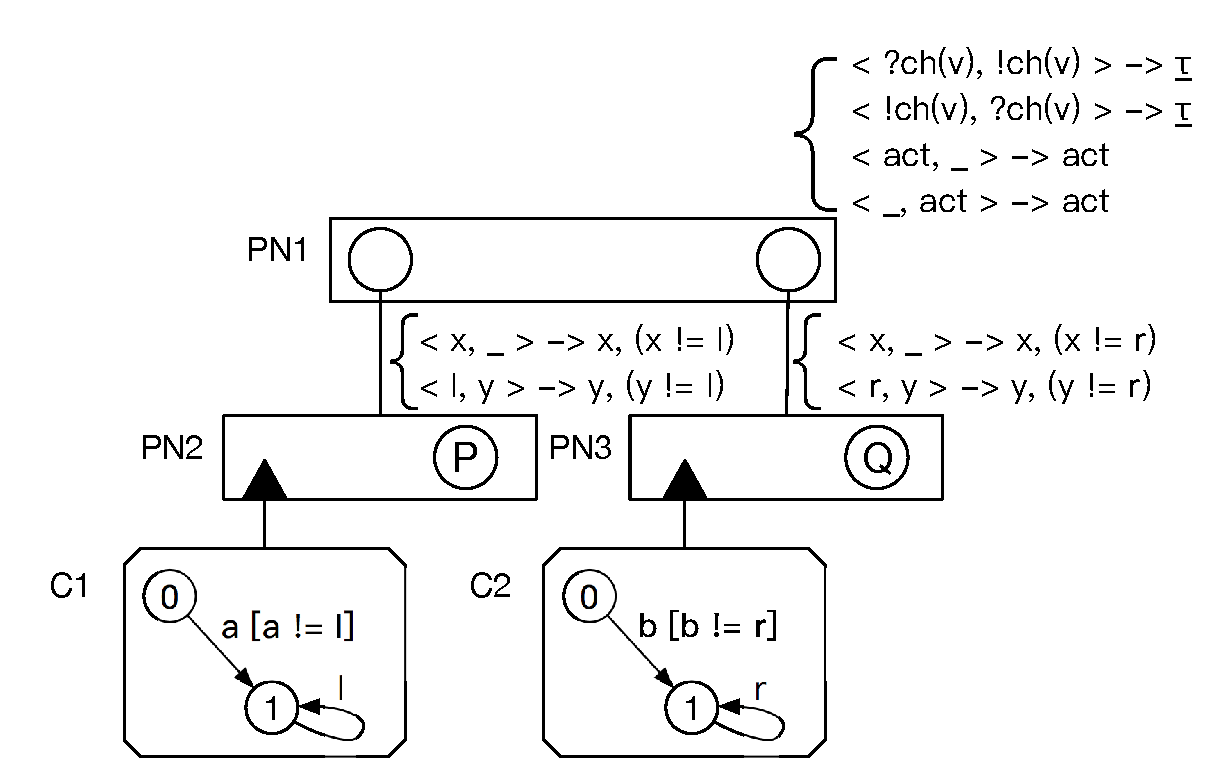
\includegraphics[width=9cm]{XFIG/CCS1}}
  \caption{The pNet encodings for CCS formula}  \label{schema:ccs-pnets}
\end{figure}

First example we choose is a formula $a.P||b.Q$, composing prefix and
parallel operators of value-passing CCS, and containing two process
variables (holes) P and Q. In Fig.~\ref{schema:ccs-pnets}, we show the encoding of this CCS
formula. The pNet has a tree-like structure.  

The root node of the tree PN1 is the top level of the pNet
  structure. It acts as the parallel operator. There are two subnets,
  noted PN2 and PN3, each representing one of the prefix
  sub-expression. Their behaviors are synchronized in their parent PN1
  according to a set of synchronization vectors, synchronizing input
  and output action from these two subnets to give out a silent action
  $\tau$ or just making the action become visible on the top level when
  one of the subnets is working alone. The vector concrete syntax is typically
  ``<act, \_ > -> act'', in which ``\_'' means that the corresponding
  subnet is not involved in this synchronization.
  There is also a difference with the usual CCS notation of
  input/output actions: in the first vector, $!ch$ and $ch$ are
  corresponding input and output channels (see next section for a more
  complete formalisation). 
  Remark that these 4
  synchronization vectors correspond faithfully to the usual SOS
  rules of CCS operational semantics.

  Each of the subnets act as one of the prefix operator.
In each of them there is a parameterized labelled transition system
(pLTS) and a hole. The pLTS is a controller managing the
changes of state of the pNet; consider C1, from its initial state the
only possible transition performs the action variable $a$; once in
state 1, the controller can perform (infinitely often) action $l$ that
is a constant action local to C1 (that must be different from any
other action of the whole system). In the node PN2, there are 2
synchronization vectors, the first one transmits to the upper level the
action $a$ (and thanks to C1, will only be activated one time); the
second one transmit any action of the hole P, but only when C1 can
perform $l$.

It should be easy to see that this pNet system encodes properly the
behavioral semantics of the corresponding CCS expression. Remark
that it is built in a systematic structural way, one pNet node
encoding each CCS operator. And it is parameterized both at the level
of actions variables (occurring within the controllers and the synchronization
vectors), and at the level of process parameters 
(holes). 

\subsection{Open pNet with Assignments in Leaves}
\begin{figure}[h]

  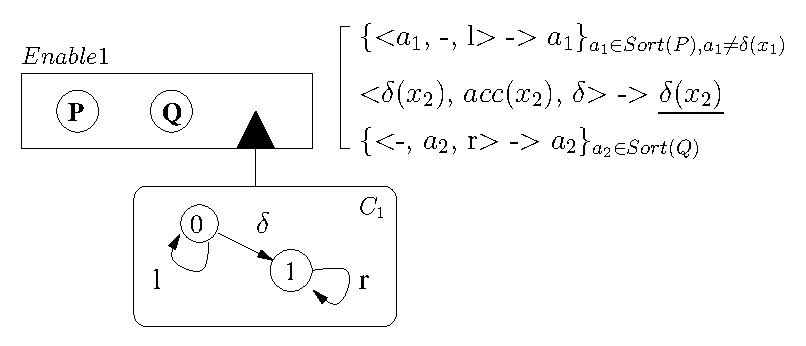
\includegraphics[width=6cm]{XFIG/Enable1.eps}
%  \hspace{0.5cm}
  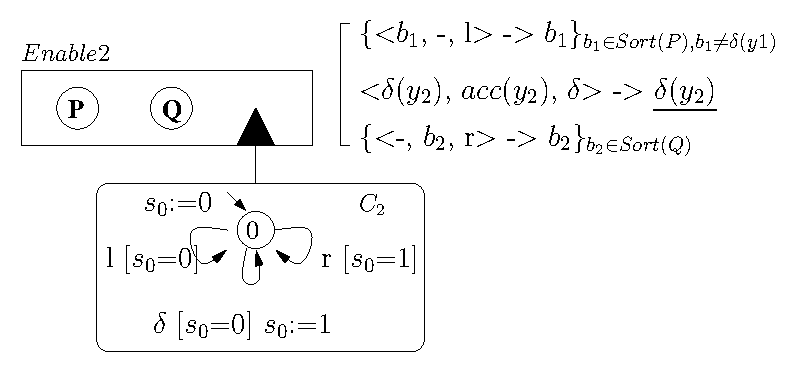
\includegraphics[width=6cm]{XFIG/Enable2.eps}
  \caption{Two pNet encodings for the Lotos Enable operator P>>Q }  \label{schema:enable-pnets}

\end{figure}

In the second running example, we want to illustrate the use of local
variables in the controller pLTSs. This example is based on the Enable
operator of the LOTOS language. For the readers not familiar with
Lotos, the pNet encodings here should be sufficient to understand the
Enable operator semantics.

In fact we give two encodings of this operator: the first one is
``state oriented'', in the sense that the controller has two states,
indicating where the control point is in the P>>Q process expression,
either in P or in Q. The transition between these occurs when process
P performs a $\delta(x)$ action, transferring the control to Q, and
sending a value $x$ at the same time. Process Q must be ready to
``accept'' this value through an $acc(x)$ action. The controller C1,
and the 3 synchronization vectors of the Enable1 pNet should be easy
to understand. Note 
that the first vector, transmitting an action $a1$ of P, can only
occur if $a1$ is not a $\delta$.

The second encoding is ``data oriented'', meaning that the state of
the node controller is encoded in the value of the pLTS state
variable(s). Here we have a single state variable $s_0$, initialized
as $0$. Its value is ``0'' when the control is on P, and ``1'' when the
control is on Q. The transitions in the pLTS have the more general
syntax: ``<action-expr> [guard] \{sequence of assignments\}''. Guards
and assignments can only use the values of variables of their source
state and values from input variables in the action expression; and a
transition can only assign variables of its target state. 
The second vector of the node ``Enable2'' also shows a
$\underline{\delta(y_2)}$ result action, where the underlined action
stands for an internal (already synchronized) action, that cannot be
further synchronized at upper levels. This is a straightforward
 generalization of the notion of internal actions, that will be
convenient for observing internal events during model-checking. 



\section{parameterized Networks (pNets): definition}
\label{section:pnets}

% \ERIC{Keep minimum defs here too be independent from FORTE}

This section introduces pNets and the notations we will use in
this paper. Then it gives the formal definition of pNet structures,
together with an operational semantics for open pNets.

pNets are tree-like structures, where the leaves are either
\emph{parameterized labelled transition systems (pLTSs)}, expressing the
behavior of basic processes, or \emph{holes}, used as placeholders
for unknown processes, of which we only specify the set of possible
actions, this set is named the \emph{sort}.
Nodes of the tree (pNet nodes) are synchronizing artifacts, using a
set of \emph{synchronization vectors} that express the possible
synchronization between the parameterized actions of a subset of the
sub-trees.


%\smallskip\noindent
\paragraph*{Notations.}
We extensively use indexed structures
over some countable indexed sets, which are equivalent to mappings over
the countable set. % . The indexes will usually be
% integers, bounded or not. Such an indexed family is
%denoted
%follows:
$a_i^{i\in I}$
%, or equivalently  $(i\mapsto a_i)^{i\in I}$
denotes a family of elements $a_i$ indexed over the
set $I$. % Such a family
% is equivalent to the mapping $(i\mapsto a_i)^{i\in I}$.
% To specify the set over which the structure is indexed,
% indexed structures are always denoted with an exponent of the form $i\in I$
% (arithmetic only appears in the indexes if necessary).
$a_i^{i\in I}$ defines both $I$ the set over which the family is
indexed (called \emph{range}), and $a_i$ the elements of the family.
E.g., $a^{i\in\{3\}}$ is the mapping with a single entry $a$ at index
$3$ ; abbreviated $(3\mapsto a)$ in the following.
When this is not
ambiguous, we shall use notations for sets, and typically write
``indexed set over I'' when formally we should speak of multisets, and
write $x\in a_i^{i\in I}$ to mean $\exists i\in I.\, x=a_i$.  An empty
family is denoted $\emptyset$. We
denote classically $\overline{a}$ a family when the indexing set is
not meaningful.  $\uplus$ is the disjoint union on
indexed sets.


\paragraph*{Term algebra.}
Our models rely on a notion of parameterized actions, that are
symbolic expressions using data types and variables. As our model aims
at encoding the low-level behavior of possibly very different
programming languages, we do not want to impose one specific algebra
for denoting actions, nor any specific communication mechanism. So we
leave unspecified the constructors of the algebra that will allow building
expressions and actions. Moreover, we use a generic {\em action interaction}
mechanism, based on (some sort of) unification between two or more action
expressions, to express various kinds of communication or
synchronization mechanisms.

\def\Talg{\mathcal{T}_{\Sigma,\P}}
Formally, we assume the existence of a term algebra $\Talg$,
where $\Sigma$ is the signature of the data and action constructors,
and $\P$ a set of variables. Within $\Talg$, we distinguish a set of
data expressions $\mathcal{E}_\P$, including a set of boolean
expressions $\mathcal{B}_{\P}$ ($\mathcal{B}_{\P}\subseteq\mathcal{E}_\P$).
On top of $\mathcal{E}_\P$ we build the action algebra
$\mathcal{A}_\P$, with $\mathcal{A}_P\subseteq\mathcal{T}_\P,
\mathcal{E}_P\cap\mathcal{A}_P=\emptyset$;
naturally action terms will use data expressions as subterms.
To be able to reason about the data flow between pLTSs, we
distinguish \emph{input variables} of the form $?x$ within terms; the function
$\vars(t)$ identifies the set of variables in a term
$t\in\AlgT$, and $iv(t)$ returns its input variables.


pNets can encode naturally the notion of input actions in value-passing CCS
\cite{Milner89} or of usual point-to-point message passing calculi, but it also allows
for more general mechanisms, like gate negotiation in Lotos, or broadcast
communications.
Formally, value-passing actions \emph{\`a la} CCS, denoted as ``?ch(x)'' and ``!ch(exp)'' in our CCS running example, stand respectively for $CCSact(i(ch),?x)$ and $CCSact(ch,exp)$, where $ch$ is a variable denoting a channel name, $?x$ is an input variable denoting the data argument received as input on $ch$, and $exp$ some data expression (containing no input variables). In our example we will use the usual CCS syntax.
%For Lotos-style
%distributed synchronization, we use synchronization vectors that encode matching data
%offers on a common gate; or 
We can also use more complex action structure such as Meije-SCCS action
monoids, like in $a.b$, $a^{f(n)}$ (see \cite{deSimone85}). The expressiveness of the synchronization constructs
will depend on the action algebra.




\subsection{The (open) pNets Core Model}
\label{section:pNets}


A pLTS is a labelled transition system with variables; variables can be
manipulated, defined, or accessed inside states, actions, guards, and
assignments. Without loss of generality and to simplify the formalization, we suppose 
here that 
variables are local to each 
state: each state has its set of variables disjoint from the others. Transmitting 
variable values from one state to the other can be done by explicit assignment. 
%Similarly, to simplify the management of variables and without loss of expressivity, we 
%suppose that transitions looping to the same state does not do assignments.
Note that we make no assumption on finiteness of the set of states nor
on finite branching of the transition relation.

We first define the set of actions a pLTS can use, let $a$
range over action labels, $\symb{op}$ are operators, and $x_i$ range over
variable names. Action terms are:
\[
\begin{array}[l]{rcl@{\quad}p{5.5cm}}
  \alpha\in\AlgA&::=&a(p_1,\ldots,p_n)&\text{action terms}\\
  p_i&::=& ?x~|~\symb{Expr}&\text{parameters (input variable or expression)}\\
  \symb{Expr}&::=& \symb{Value}~|~x~|~\symb{op}(\symb{Expr}_1,..,\symb{Expr}_n)&\text{Expressions}
\end{array}
\]
The input variables in an action term are those marked with a
$\symb{?}$.
We additionally suppose that each input variable does not
appear somewhere else in the same action term:
$p_i=?x\Rightarrow\forall j\neq i.\, x\notin \vars(p_j)$

\begin{definition}[pLTS]
\label{pLTS}
A pLTS is a tuple
$pLTS\triangleq\mylangle S,s_0, \to\myrangle$ where:
\begin{itemize}
\item[$\bullet$]
$S$ is a set of states.
\item[$\bullet$]
$s_0 \in S$ is the initial state.
%\item[$\bullet$]
 %Variables in
%$\iv(\alpha)$ are assigned by the action, other variables can be assigned
%by the additional assignments.
\item[$\bullet$] $\to \subseteq S \times L \times S$ is the transition relation and 
$L$ is the set of labels of the form
$\langle \alpha,~e_b,~(x_j\!:= {e}_j)^{j\in J}\rangle$,
where $\alpha \in\AlgA$ is a parameterized action, $e_b \in
\AlgB$ is a guard, and the variables $x_j\in P$
are assigned the expressions $e_j\in \AlgE$.
If 
$s \xrightarrow{\langle \alpha,~e_b,~(x_j\!:= {e}_j)^{j\in
		J}\rangle} s'\in \to $ then $\iv(\alpha)\!\subseteq\! \vars(s')$, 
		$\vars(\alpha)\backslash \iv(\alpha)\!\subseteq\! \vars(s)$, 
		$\vars(e_b)\!\subseteq\! \vars(s')$, and
		$\forall j\!\in\! J .\,\vars(e_j)\!\subseteq\! \vars(s)\land 
		x_j\!\in\!\vars(s')$. %,  and $s= s'\Rightarrow J=\emptyset$. 
\item[$\bullet$]
The $x_j$ here are $state\ variables$ of state $s'$. $State\ variables$ can only be modified by the assignment in the transitions targetting its owner state. A global state variable of a pLTS is a variable $x$ satisfying $\forall s\!\in\! S .\, x\!\in\! \vars(s)$.


\end{itemize}
\end{definition}

Now we define
pNet nodes, as constructors for hierarchical behavioral structures.
A pNet has a set of sub-pNets that can be either pNets or pLTSs, and a
set of Holes, playing the role of process parameters.

A composite pNet consists of a set of sub-pNets exposing
a set of actions, each of them triggering internal actions in each of
the sub-pNets. The synchronization between global actions and
internal actions is given by  \emph{synchronization vectors}: a
synchronization vector synchronises one or several internal actions, and
exposes a single resulting global action.
Actions involved at the pNet level (in the synchronization vectors) do
not need to distinguish between input and output
variables. Action terms for pNets are defined as follows:
\[\begin{array}[l]{rcl@{\quad}l}
  \alpha\in \AlgAS &::=&a(Expr_1,\ldots,Expr_n)
\end{array}
\]



\begin{definition}[pNets]\label{def-pnets}
A pNet is a hierarchical structure where leaves are pLTSs and holes:\\
$\pNet\triangleq pLTS~|~\mylangle \pNet_i^{i\in I}, S_j^{j\in J}, \symb{SV}_k^{k\in K}\myrangle$
where
\begin{itemize}
\item[$\bullet$] $I \in \I$ is the set over which sub-pNets are indexed.
\item[$\bullet$] $\pNet_i^{i\in I}$ is the family of sub-pNets.
%  $\pNet_i^{i\in I}$ is a family of sub-pNets where $I\in\I_\P$ is the set over which sub-pNets are indexed.

\item[$\bullet$] $J\in\I_\P$ is the set over which holes are indexed.
$I$ and $J$ are \emph{disjoint}: $I\cap J=\emptyset$,  $I\cup J\neq\emptyset$
\item[$\bullet$] $S_j \subseteq \AlgAS$ is a set of action terms, denoting the $\Sort$ of
hole $j$.

\item[$\bullet$] $\symb{SV}_k^{k\in K}$ is a set of
  synchronization vectors ($K\in\I_\P$). $\forall k\!\in\! K,
  \symb{SV}_k\!=\!\alpha_{l}^{l\in I_k \uplus J_k}\to\alpha'_k$ where
  $\alpha'_k\in \mathcal{A}_\P$, $I_k\subseteq I$, $J_k\subseteq J$,
  $\forall i\!\in\!
  I_k.\,\alpha_{i}\!\in\!\Sort(\pNet_i)$,  $\forall j\!\in\!
  J_k.\,\alpha_{j}\!\in\!S_j$, and $\vars(\alpha'_k)\subseteq \bigcup_{l\in I_k\uplus 
  J_k}{\vars({\alpha_l})}$. The global action of a vector $\symb{SV}_k$ is
$\Label(\symb{SV}_k) = \alpha'_k$.


\end{itemize}
\end{definition}

The preceding definition relies on the auxiliary functions below:

\begin{definition}[Sorts, Holes, Leaves of pNets]
  \begin{itemize}
  \item The sort of a pNet is its signature, i.e. the set of actions it can
perform. In the definition of sorts, we do not need to distinguish
input variables (that specify the dataflow within LTSs), so for
computing LTS sorts, we use a substitution operator\footnote{$\subst{y_k\gets x_k}^{k\in K}$ is the parallel substitution 
operation.} to remove the
\emph{input marker} of variables. Formally:
\[
\begin{array}{l}
\Sort(\mylangle S,s_0, \to\myrangle) = \{\alpha\subst{x \gets ?x| 
x\in\symb{iv}(\alpha)}|s \xrightarrow{\langle \alpha,~e_b,~(x_j\!:= {e}_j)^{j\in
		J}\rangle} s'\in \to \} \\ \Sort(\mylangle
\set{\pNet}, \set{\symb{S}}, \set{\symb{SV}}\myrangle) =\{\alpha'_k |\, \alpha_j^{j\in J_k}\to\alpha'_k\in\set{\symb{SV}}\}
\end{array}
\]

\item
The set of holes of a pNet is defined inductively; the sets of holes
in a pNet node and its subnets are all disjoint:
  \[\begin{array}{l}
\Holes(\mylangle S,s_0, \to\myrangle) \!=\! \emptyset \\
\Holes(\mylangle \pNet_i^{i\in I}\!,S_j^{j\in J}\!, \overline{\symb{SV}}\myrangle) =J\cup{\displaystyle \bigcup_{i\in I}\Holes(\pNet_i)}\\
\forall i\in I.\, \Holes(\pNet_i)\cap J=\emptyset\\
\forall i_1,i_2\in I.\,i_1\neq i_2\Rightarrow  \Holes(\pNet_{i_1})\cap\Holes(\pNet_{i_2})=\emptyset
\end{array}\]
\item
The set of leaves of a pNet is the set of all pLTSs occurring in the structure, defined inductively as:
\[\begin{array}{l}
\Leaves(\mylangle S,s_0, \to\myrangle) \!=\! \{ \mylangle S,s_0, \to\myrangle \}\\
\Leaves(\mylangle \pNet_i^{i\in I}\!,S_j^{j\in J}\!, \overline{\symb{SV}}\myrangle) = {\displaystyle \bigcup_{i\in I}\Leaves(\pNet_i)}
\end{array}\]
\end{itemize}
\end{definition}

A pNet $Q$ is \emph{closed} if it has no hole: $\Holes(Q)=\emptyset$; else it
is said to be \emph{open}.


%% \begin{figure}[t]
%% \begin{minipage}{6.1cm}

%%   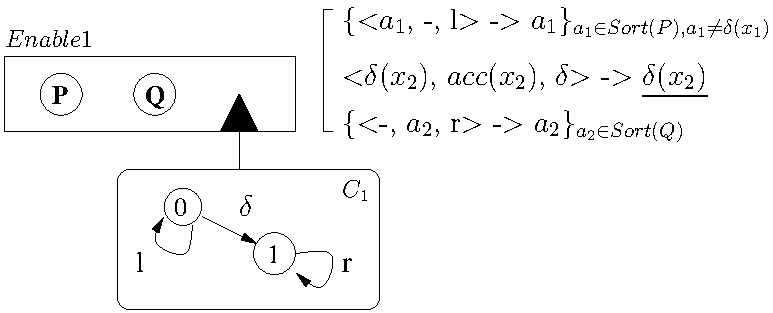
\includegraphics[width=\linewidth]{XFIG/Enable1}
%%   \\[1.3ex]
%%  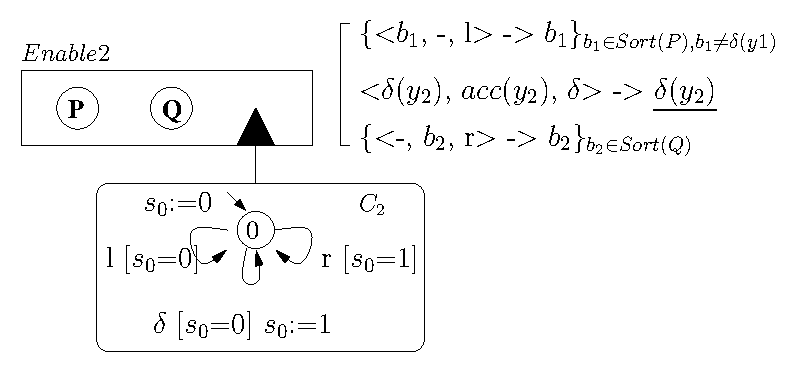
\includegraphics[width=\linewidth]{XFIG/Enable2}
%%   \caption{Two pNet encodings for  Enable }  \label{schema:enable-pnets}
%% \end{minipage}
%%   \hspace{2mm}
%% \begin{minipage}{6cm}
%%   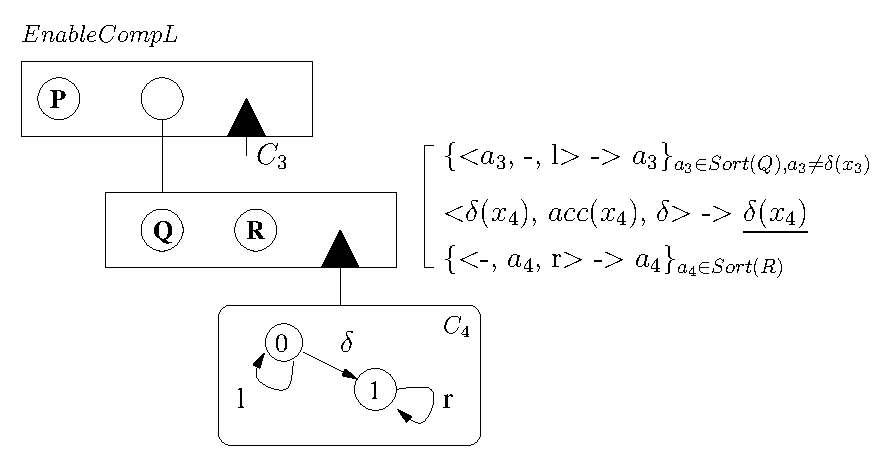
\includegraphics[width=\linewidth]{XFIG/P-QR}
%%   \caption{Composed pNet for ``P>>(Q>>R)''}  \label{schema:enable-composed}
%% \end{minipage}

%% \end{figure}





\section{Operational Semantics for Open pNets}
\label{section:op-semantics}



The semantics of open pNets will be defined  as an open automaton. An open
automaton is an automaton where each transition composes transitions of several LTSs with
action of some holes, the transition occurs if some predicates hold, and can involve a 
set of state modifications.

\begin{definition}[Open transitions]
	\label{def:OpenTransitions}
	An \emph{open transition} over a set  $(S_i,s_{0 i}, \rightarrow_i)^{i\in
	I}$ of LTSs, a
	set $J$ of holes with sorts $Sort_j^{j\in J}$, and a set of states $\mathcal{S}$ is a structure of the form:	
	\begin{mathpar}
	\inferrule*[myfraction=\reddottedrule]
	{\{s_i~{\xrightarrow{a_i}}_i ~s_i^{\prime}\}^{i\in I},
		\{\xrightarrow{b_j}_j\}^{j\in J}, \Pred, \Post}
	{s \xrightarrow {v}s'}
	\end{mathpar}
	Where $s, s'\in\mathcal{S}$ and for all
        $i\in I$, $s_i{\xrightarrow{a_i}}_i s_i^{\prime}$ is a transition of the
	LTS $(S_i,s_{0 i}, \rightarrow_i)$, and $\xrightarrow{b_j}_j$
        is a transition of the hole $j$, for any action $b_j$ in the
        sort $Sort_j$. \Pred\ is a predicate
	over the different variables of the
	terms, labels, and states $s_i$, $b_j$, $s$, $v$. \Post\ is a set of equations that 
	hold \emph{after the open transition}, they are represented as a substitution of the 
	form $\{x_k\gets e_k\}^{k\in K}$ 
	where $x_k$ are variables of $s'$, $s'_i$, and $e_k$ are expressions over the other 
	variables of the open transition.
\end{definition}

\begin{example}\emph{An open-transition.}
  \label{OT:ccs-composed}
%  \TODO{ERIC: change for an OT of CCS example}
The \texttt{CCS} pNet of Fig. \ref{schema:ccs-pnets} has 2 controllers and 2 holes. We show its full open Automaton in section \ref{section:full-result}, it has 16 open transitions. We detail 3 of them here:

 \smallskip
 $  OT_1  = \openrule{
                       0 \xrightarrow{a}_{C_1} 1 ~~
                       0 \xrightarrow{b}_{C_2} 1  ~~
                       \{\}               ~~
                 [ a\neq l \land b\neq r \land a=?ch(v) \land b=!ch(v) ]              
                      }
     {\ostate{00} \xrightarrow{\underline{\tau}} \ostate{11}}$
     
 $ OT_3  = \openrule{
                       0 \xrightarrow{a}_{C_1} 1 ~~
                       \{\}               ~~
                 [ a\neq l  ]              
                      }
     {\ostate{10} \xrightarrow{a} \ostate{10}} $
     
$  OT_{11}  = \openrule{
                          1 \xrightarrow{l}_{C_1} 1 ~~
                       0 \xrightarrow{b}_{C_2} 1 ~~
                       \{ \xrightarrow{hb_P}_{P} \}               ~~
                 [ a\neq l \land b\neq r \land hb_P=?ch(v) \land b=!ch(v) ]              
                      }
     {\ostate{10} \xrightarrow{\tau} \ostate{11}}
  $
\end{example}

The first open transitions listed, $OT_1$ and $OT_3$, only involve
possible actions from the prefix operators, respectively communication
between the two prefixes, if actions $a$ and $b$ are matching emit and
receive actions on the same channel; or simple propagation of action
$a$ from the left prefix, with no special constraint other than being
different from the local $l$ action of pLTS $C_1$.

Remark the structured states in the conclusion of these rules: both
start in state $\ostate{00}$, where both $C_1$ and $C_2$ are in their
initial states. They end in different structured states, because in
$OT_1$ both pLTS chage states, meaning that the control has gone
respectively to processes $P$ and $Q$, consuming actions $A$ and $B$,
while in $OT_3$ only $C_1$ has moved.

The last open transition $OT_{11}$ starts in state $\ostate{10}$, with
control at $P$ on the left, and action $b$ on the right. So these two
can communicate, e.g. here if $b$ is an emission, and the action of hole
$P$ is the matching reception.

\begin{definition}[Open automaton]
	\label{def:open-automaton}
	An \emph{open automaton} is a structure\\ $A =
	<LTS_i^{i\in I},J,\mathcal{S},s_0,\mathcal{T}>$ where:
	\begin{itemize}
		\item[$\bullet$]  $I$ and $J$ are  sets of indices,
		\item[$\bullet$]  $LTS_i^{i\in I}$ is a family of LTSs,
		\item[$\bullet$]   $\mathcal{S}$ is a set of states and $s_0$ an initial state
		among $\mathcal{S}$,
		\item[$\bullet$] $\mathcal{T}$ is a set of open transitions and for each
		$t\in \mathcal{T}$ there exist $I'$, $J'$ with $I'\subseteq I$, $J'
		\subseteq J$, such that $t$ is an open transition over $LTS_i^{i\in I'}$, $J'$,
		and  $\mathcal{S}$.
		
	\end{itemize}
\end{definition}
	

%
%Then the semantics of a pNet is characterized by a set of {\em open
%transitions}, where the hypotheses on process parameters are
%replaced by 1) transitions of the pLTSs at the leaves, and 2) formal
%hypotheses on the transitions of the holes. A {\em predicate} is used
%to relate the parameters and names appearing in the actions of the
%leaves and the holes involved in the rules, but also appearing in  the resulting action.


\begin{definition}[States of open pNets]\label{def-states}
  A state of an open pNet is a tuple (not necessarily finite) of the
  states of its leaves (in which we denote tuples
  in structured states as $\triangleleft\ldots\triangleright$ for better readability).

  For any pNet p, let $\overline{Leaves} = \mylangle S_i,{s_i}_0, \to_i\myrangle^{i \in L}$ be the set of pLTS at its leaves,
  then $States(p) = \{\triangleleft s_i^{i\in L}
  \triangleright| \forall i\in L. s_i \in S_i\}$.
A pLTS being its own single leave:
  $States(\mylangle S,s_0, \to\myrangle) = \{\triangleleft s \triangleright| s \in S\}$.

The initial state is defined as:
$InitState(p) = \triangleleft {{s_i}_0}^{i\in L}  \triangleright$.
\end{definition}

%% \begin{example} \emph{State of a pNet}
%%   The states of pNet \texttt{EnableCompL} are:
%%   $\triangleleft 00 \triangleright, \triangleleft 10 \triangleright, \triangleleft 11 \triangleright$
%% \end{example}

\paragraph{Predicates:}
Let
$\mylangle\overline{\pNet},\overline{S},\symb{SV}_k^{k\in K} \myrangle$
be a pNet. Consider a synchronization vector $SV_k$, for $k\in K$. We define a
predicate $\Pred$ relating
the actions of the involved sub-pNets and the resulting actions. This predicate verifies:
\[\Pred(SV_k, a_i^{i\in I}, b_j^{j\in J}, v)\Leftrightarrow
\begin{array}{l}
\exists {(a'_i)}^{i\in I},
{(b'_j)}^{j\in J},v'.\, SV_k={(a'_i)}^{i\in I}, {(b'_j)}^{j\in J}\rightarrow v'
\\~~\land
\forall i\in I.\, a_i=a'_i\land \forall j \in J.\, b_j=b'_j \land v=v'
\end{array}\]
In any other case (if the action families do not match or if there is no valuation of
variables such that the above formula can be ensured) the predicate is undefined.

This definition is not constructive but it is easy to build the predicate constructively
by brute-force unification of the sub-pNets
actions with the corresponding vector actions, possibly followed by a simplification
step.


We build the semantics of open pNets as an open automaton where LTSs are the pLTSs at
the leaves of the pNet structure, and the states are given by 
Definition~\ref{def-states}. The open transitions first
 project the global state into states of the leaves, then apply
pLTS transitions on these states, and compose them with the sort of the holes. %The pNet
%structure does not appear in the open-automaton, only the
%set of Holes and the set of Leaves.
The semantics   regularly instantiates \emph{fresh} variables, and uses a
\emph{clone} operator that clones a term replacing each variable with a
fresh one.

The semantic of the open pNets is already defined as an open automaton in \cite{henrio:Forte2016} using open transitions to present the transitions of its global states.
\begin{definition}[Operational semantics of open pNets]
  \label{def:operationalSemantics}
  The semantics of a pNet $p$ is an open automaton $A = <Leaves(p),J,\mathcal{S}, s_0,
  \mathcal{T}>$ where:
  \begin{itemize}
    \item $J$ is the indices of the holes: $Holes(p)= H_j^{j\in J}$.
    %  \item $\overline{L}^L = Leaves(p), \overline{H}^J = Holes(p)$
    \item $\overline{\mathcal{S}} = States(p)$ and $s_0 = InitState(p)$
    \item $\mathcal{T}$ is the smallest set of open transitions
    satisfying the rules below:
  \end{itemize}
  
  The rule for a pLTS $p$  checks that the guard 
  is verified and transforms assignments into post-conditions:
  
  \begin{description}
    \item[{\bf Tr1:}]
    $\inferrule
    { s \xrightarrow{\langle \alpha,~e_b,~(x_j\!:= {e}_j)^{j\in
          J}\rangle} s'\in \to  \\
      {\tt fresh}(v) \\
      Pred = ~e_b \land (\alpha = v)
    }
    { p = \mylangle  S,s_0, \to \myrangle
      \models
      \inferrule*[myfraction=\reddottedrule]
      {\{s \xrightarrow{\alpha}_p s'\} ,\emptyset ,
      Pred,\left\{x_j\gets e_j\right\}^{j\in J}}
      {\ostate{s} \xrightarrow{v} \ostate{s'}}
    }
    $
  \end{description}
% Note that this note is greatly simplified by the fact that variables are local to 
% thread; introducing global state variables or accepting loops to the same 
% state would 
% require to reason 
% on the scope of 
% each variables, and to introduce additional variables to handle the several occurence 
% of the same pLTS variable in the predicates. Indeed the constraints on pLTS 
% transitions 
% ensure that the same variable never appears both on the left and on the right of the 
% equations of a predicate.
  
  The second rule deals with pNet nodes: for each possible
  synchronization vector applicable to the rule subject, the premisses
  include one {\em open transition} for each sub-pNet involved, one possible
  {\em action} for each Hole involved, and the predicate relating these
  with the resulting action of the vector.
  A key to understand this rule is that the open transitions are
  expressed in terms of the leaves and holes of the pNet structure,
  i.e. a flatten view of the pNet: e.g. $L$ is the index set of the
  Leaves, $L_k$ the index set of the leaves of one subnet, so all $L_k$
  are disjoint subsets of $L$. Thus the states in the open transitions,
  at each level, are tuples including states of all the
  leaves of the pNet, not only those involved in the chosen
  synchronization vector.
  
  \begin{description}
    \item[{\bf Tr2:}]
  \end{description}
  
  \noindent
    $\inferrule
    {k\!\in\! K \\ SV\!\!= \!clone(SV_k) \!=\! \alpha_m^{m \in I_k\uplus J_k} \!\to\! 
    \alpha'_k, G_k \\
      Leaves(p) \!=\! \pLTS_l^{l\in L} \\     
      \forall m\in I_k.
      \pNet_m \models
      \inferrule*[myfraction=\reddottedrule]
      {\{s_{i}\xrightarrow{a_{i}}_i s_{i}'\}^{i\in I_m^\prime},
      \{\xrightarrow{b_{j}}_j\}^{j\in J'_m}, \Pred_m, \Post_m}
      {\ostate{s_{i}^{i \in L_m}} \xrightarrow {v_m}
        \ostate{s_{i}^{\prime\ i \in L_m}}}
      %\land
      %Leaves(\pNet_m) = \overline{pLTS}^{L_k})
      \\
      I' = \biguplus_{m\in I_k}\!\! I_m'
      \\ J' = \biguplus_{m\in I_k}\!\! J'_m \uplus J_k  \\
      \Pred = \bigwedge_{m\in I_k}\!\! \Pred_m \land
      \Pred(SV,v_m^{m\in I_k},b_j^{j\in J_k},v)\\
      \forall j\!\!\in\!\! J_k. {\tt 
        fresh}(b_j) \\ {\tt fresh}(v) \\ 
      \forall i\in
      L\backslash I'.\,s'_i=s_i 
    }
    {p = \mylangle \pNet_i^{i\in I}, S_j^{j\in J}, \symb{SV}_k^{k\in K}\myrangle
      \models
      {\inferrule*[myfraction=\reddottedrule]
        {\{s_i\xrightarrow{a_i}_i s_i^{\prime}\}^{i\in I^\prime},
        \{\xrightarrow{b_j}_j\}^{j\in J^\prime}, \Pred, \uplus_{m\in I_k} 
        \Post_m}
        {\ostate{s_i^{i\in L}} \xrightarrow {v}
          \ostate{s_i^{\prime i\in L}}}
      }
    }
    $

  \medskip  
\end{definition}

%
\begin{figure}[tb]
\begin{mathpar}
  \small
  \inferrule
    {\inferrule
      {
          \inferrule
              {1 \xrightarrow {l}_{C_1} 1}
              {C_1
                \models
                \openrule
                      {1 \xrightarrow{l}_{C_1} 1}
                      {\ostate{1}\xrightarrow{1}\ostate{1}}
              }
        }
        {\textrm{a:P}
          \models
            \openrule{
              1 \xrightarrow {l}_{C_1} 1,\,
              \{\xrightarrow{b_P}_P\},\, b_P\neq l}
                      {\ostate{1}\xrightarrow{b_P}\ostate{1}}
        }\\
%      \sm{fresh}v         \\
      \inferrule%*[right={L_1}]
        {
          \inferrule
              {0 \xrightarrow{b}_{C_2} 1}
              {C_4
                \models
                \openrule
                      {0 \xrightarrow{b}_{C_2} 0,\, b\neq r}
                      {\ostate{0}\xrightarrow{b}\ostate{1}}
              }
        }
        {
          \textrm{b:Q}\models
              \openrule
                  { 0 \xrightarrow {b}_{C_2} 1,\, \ b\neq r}
                  {\ostate{0}\xrightarrow{b}\ostate{1}}
        }   
    }
    {
     \textrm{PN1}
     \models
        \openrule{
                       1 \xrightarrow{l}_{C_1} 1 ~~
                       0 \xrightarrow{b}_{C_2} 1 ~~
                       \{ \xrightarrow{b_P}_{P} \}               ~~
                 [ a\neq l \land b\neq r \land b_P=?ch(v) \land b=!ch(v) ]              
                      }
     {\ostate{10} \xrightarrow{\tau} \ostate{11}}
      }\vspace{-4ex}
\end{mathpar}
  \caption{Proof of  $OT_{11}$ (with interaction of processes $P$ and action $b$) for ``a.P||b.Q''}
  \label{usingrules:OT11}
\end{figure}

\begin{example} \emph{Using the operational rules to compute
    open-transitions}
  In Fig. \ref{usingrules:OT11} we show the deduction tree used to construct and prove the 
  open transition $OT_{11}$ of \texttt{CCS} (see example page
  \pageref{OT:ccs-composed}).
%  \TODO{Eric: change for a deduction tree of CCS expression}
The proof tree uses TR1 twice, for the $l$ transition of $C_1$ and for the
  $b$ transition of $C_2$, then uses an action $b_P$ of hole $P$, and
  combines the results using the second vector of the PN2 sub-pNet, and
  the third vector of the top node. This yields a final $\tau$
  transition. The deduction tree in the figure shows how the
  predicates are generated in this process. 

\end{example}

    

%% Note that while the scenario above is expressed as a single
%% instantiation of the possible behaviours, the constructions below are
%% kept symbolic, and each open-transition deduced expresses a whole family of
%% behaviours, for any possible values of the variables.

\paragraph{Variable management.}
The variables in each synchronization vector are considered local:
for a given pNet expression, we must have fresh local variables for
each occurrence of a vector (= each time we instantiate rule
Tr2). Similarly the state variables of each copy of a
given pLTS in the system, must be distinct, and those created for each
application of Tr2 have to be fresh and all distinct. 
This will be implemented within the open-automaton generation algorithm,
e.g. using name generation using a global counter as a suffix.


\subsection{Presentation of algebra}
One of the important goal of the Open pNet framework is to provide us
with a model able to express the semantics of many different algebras
or languages. In particular, as we have seen in section
\ref{section:pnets}, the \emph{term algebra} used to express the
action expressions and the data in their parameters is left open in
the pNet formalisation.

So, for a given language, we now need to specify its data and action
domains, giving them an abstract syntax (sorts, constructors, operators,
and predicates). We call this a \emph{Presentation}.
We also define a concrete syntax, that will be used for
pretty-printing, but also for translating the presentation, and the
predicates, into Z3 syntax. 

An algebra presentation contains:
\begin{itemize}
	\item Sorts: Constants sets of the algebra, types of the data
          and actions. 
	\item Operators: Operators used to construct action
          expressions (including their data parameters); they are
          constructors of data and action sorts, but also predicates
          over these objects.
        \item Constants: The satisfiability solver need to know which
          actions in the pLTS behaviors are constants (like the $l$,
          $r$ local actions of the controllers in the CCS example). So
          for a given pNet system, the Action sort will include all
          these constants.
\end{itemize}

\paragraph{Sorts}
Ownership of the variables and constants in a pNet acting as actions
or data is probably various. Sorts are represented by their name. The
sort of actions is built by the constant actions. Sorts here act as
sets of actions for pNet, pLTS or 
holes. There \emph{must} be one sort for actions, and eventually
several others for the types of data parameters. Sorts for integer
and boolean are implicitly declared. 

\QIN{
In the CCS example, we have a sort for actions called $Action$:
}

\[ Action = \{ l, r\} \]

\paragraph{Operators}
We need introduce operators for building expressions, of both action
and data sorts, when encoding the 
algebra into pNets. So that is needed to know about the input and
output of the operators used in the expressions from those
algebra. The input and output should belong to the sorts of the
pNet. When there are $k$ sorts in this pNet, the structure of a
$n$-ary operator is vector as $< Sort_{i_1}, ... , Sort_{i_n} >
\rightarrow Sort_j , i_1 , ... , i_n, j \in [0..k] $.

\QIN{For instance, in our CCS running example, there is the action expression $!ch(v)$ using an operator $!$ presenting the ``$EMIT$'' action in CCS. We only use a sort called $Action$ to involve all the constant actions or action expressions in pNets and other parameters such as channel $ch$ or variable $v$ are all integers. So here we treat $EMIT$ as a binary operator with the format like:
}

 \[ < Int, Int > \rightarrow Action . \]

\paragraph{Implementation of the expression meta-model}
The VerCors platform uses Ecore and EMF to define the structure of
both pNets and actions algebras. There exists a predefined set of
action and data expressions classes, including boolean, integer and
action expressions, with predefined variables, literal (constants),
and operators. Operators can be categorized into unary, binary and
N-ary operators.
The original version of VerCors did not allow to extend these classes,
we have modified its architecture so that a user can extend them,
defining more elements for his specific algebra.

In Fig~\ref{schema:expression-pnets}, we show the Expression class we
improved, including extensions for CCS and LOTOS.

\QIN{The translation of the presentation in the Z3 SMT solver will be given later.
}

\begin{figure}[t]
  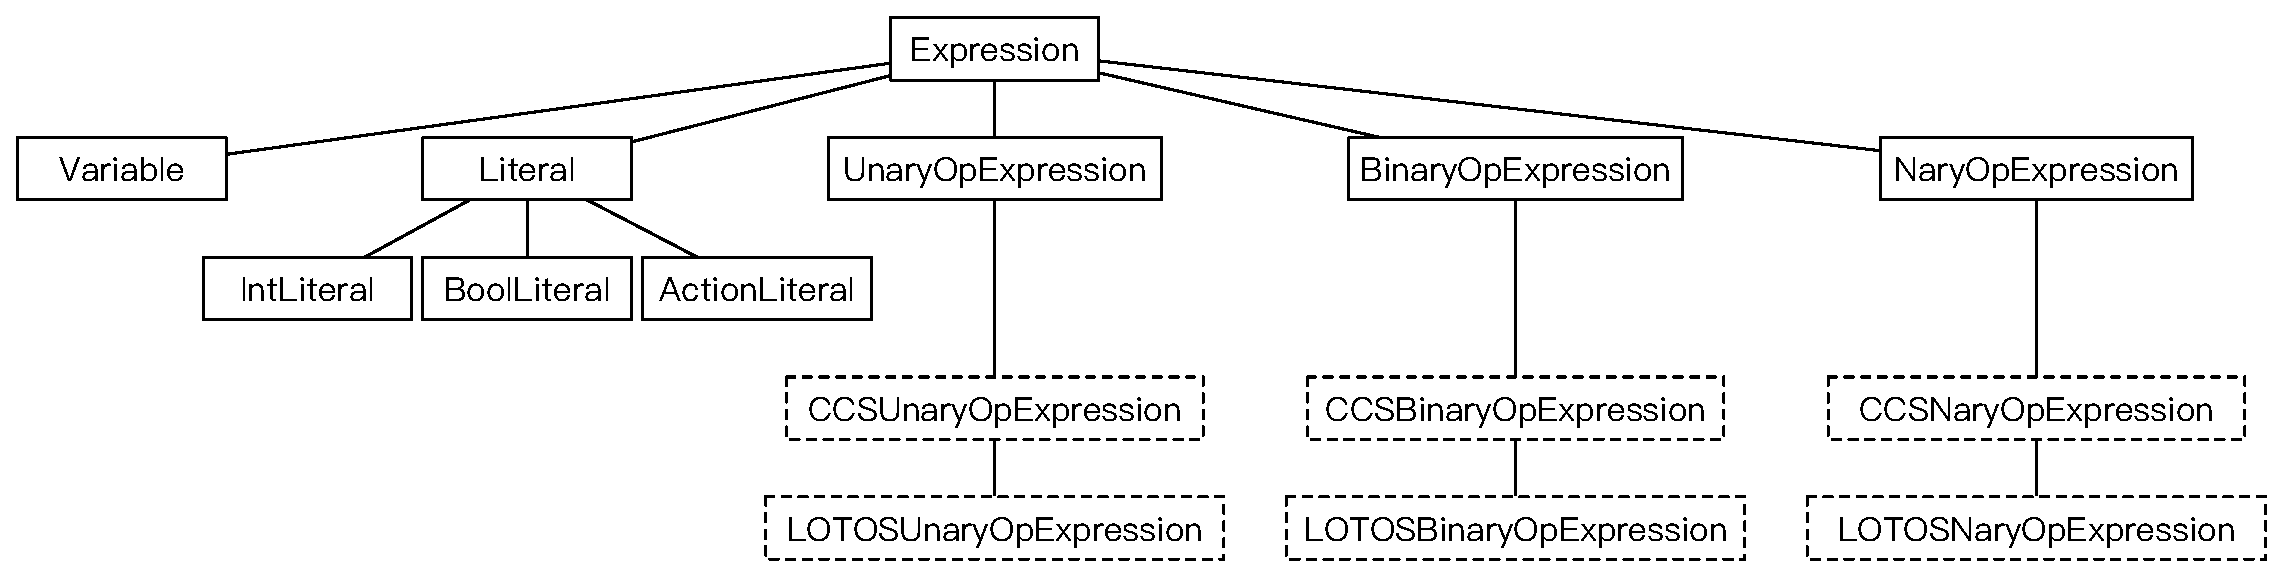
\includegraphics[width=\linewidth]{XFIG/Expression}
  \caption{The architecture of Expression class}  \label{schema:expression-pnets}
\end{figure}

%\TODO{give an example of user-defined sorts/operators, and tell that
%  you will give it's translation into Z3 in section 5.4}

\subsection{Computing and using open automata}
In this section we present an algorithm to construct the open
automaton representing the behaviour of an open pNet, and we prove that
under reasonable conditions this automaton is finite.

\begin{alg}[behavioral semantics of open pNets: Sketch]
This is a standard residual algorithm over a set of open-automaton
states, but where transitions are open transitions
constructively ``proven'' by deduction trees.

1) Start with a set of unexplored states containing the initial state
of the automaton, and an empty set of explored states.

2) While there are unexplored states:

2a) pick one state from the unexplored set and add it to the explored
set. From this state
build all possible deduction trees by application of the structural
rules Tr1 and Tr2, using all applicable combinations
of synchronization vectors.

2b) For each of the obtained deduction trees, extract the resulting
open-transition, with its predicate and \Post\ assignments by exploring the structure of 
the pNet.

2c)
The predicate is submitted to Z3 for checking satisfiability. If it is
NOT satisfiable, the resulting OT is discarded. This will minimize the
number of 
resulting transitions. Then a reachability check could potentialy
prune the state space.

For each open-transition,  add the transition in the outgoing transitions of
the current state, and add the
resulting state in the unexplored set if it is not already in the
explored set.

\end{alg}



To have some practical interest, it is important to know when this
algorithm terminates. The following theorem shows that an open-pNet
with finite synchronization sets, finitely many leaves and
holes, and each pLTS at leaves having a finite number of states and
(symbolic) transitions, has a finite automaton:

\begin{theorem}[Finiteness of open-automata.]\\
Given an open pNet $\mylangle \overline{\pNet},\overline{S}, \symb{SV}_k^{k\in K}\myrangle$ with leaves $pLTS_i^{i\in L}$ and holes $Hole_j^{j\in
  J}$, if the sets $L$ and $J$ are finite, if the synchronization vectors of all pNets 
  included in  $\mylangle \overline{\pNet},\overline{S}, \symb{SV}_k^{k\in K}\myrangle$ 
  are finite, and if
$\forall i \in L.\, finite{(states(pLTS_i))} \text{ and } pLTS_i$
has a finite number of state variables, then Algorithm 1 terminates
and produces an open automaton 
$\mathcal{T}$ with finitely many states and transitions.

The proof can be found in \cite{henrio:Forte2016}.

% Given an open pNet $\mylangle \overline{\pNet},\overline{S}, \symb{SV}_k^{k\in
%     K}\myrangle$ with leaves $pLTS_i^{i\in L}$ and holes $Hole_j^{j\in
%   J}$,
% build its semantics as in algorithm 1.

% We have:

% $$ finite{(L)} \land finite{(J)} \land \forall i \in L finite{(\{s_i\})}
%   \to finite{(\mathcal{T})}$$
\end{theorem}

\section{Implementation}
\label{section:implementation}
The VerCors platform uses (closed) pNets as the intermediate language
for some high-level language or graphical formalism to be translated
into both input for a 
model-checker and for generating executable code automatically \cite{HKM-FASE16}.
% to ease the
% specification from non-expert users, compiling it
%from those language or graphical formalism in the pNet API.

In our prototype we start directly with open pNets expressed
programmaticaly, using the pNet API (graphical editors may be added
later). From these, we compute
the open automaton of an open pNet by directly
implementing the sketch showed before. However, we made some
modifications due to implementation choices:
\begin{itemize}
  \item Steps 2a-2b are merged, applying Tr2 from the
premisses OTs from subnets to generate open transitions without
explicitely constructing the deduction tree.
  \item We defined a general naming schema for implementing the fresh 
and clone functions to rename all the variable to make them unique, but also
readable enough for debugging purpose.
  \item Besides that, we also have designed a management of state variables and
    assignments throughout the whole computation.
  \item Satisfiability check is done only at
top level of the open-transition construction. An alternative would be
to submit the satisfiability check to the SMT solver at each level of
the hierarchical OT construction, potentially reducing the overall number of
combinations. But the submission to the SMT engine is costly, and more
complexity analysis is required before deciding if this would be
worthwhile. 
\end{itemize}

In the following sections, we detail:
\begin{itemize}
\item The structure of fresh variable names.
\item The details of the implementation for step 2a-2b, refined into:
  \subitem combining all possibilities of subnets activity/inactivity,
  \subitem matching each combination with synchronization vectors.
\item Management of local variables of pLTSs.
\item Pruning of unsatisfiable open transitions using the Z3 SMT solver.
\end{itemize}

  
  

\subsection{Fresh variables}

The variables in each synchronization vector are considered local, so
does the variables of an open transition such as its hole behaviors
and its result action. So we want rename the variables to make them
unique on every occurrence of a vector. Similarly, the name given to
the hole behaviors for each hole or the result action for each open
transition must be distinct. At the same time, we also hope them still
readable. Here we have defined a structure for the name of the fresh
variables, the variables renamed with a regular format by the function
fresh(). 


More precisely, the fresh function generates a new name adding a
suffix after the original name. The suffix contains three parts
combined by a colon.  


\begin{definition}[Fresh variable]\label{fresh-variable}
The format of \emph{fresh variable} (renaming) is defined as:
$$\emph{prefix : tree\ index\ :\ counter}$$
\begin{itemize}
   \item[$\bullet$] $prefix$ is a default internal name for the variable. So far the internal name can be  sva (SV action), ra (result action), hb (hole behavior).
   \item[$\bullet$] $tree\ index$ is the index of the node in the tree-like structure of the pNet.
   \item[$\bullet$] $counter$ is the current value of the corresponding counter.
\end{itemize}
\end{definition}

%\TODO{Option: Add the process and the vector ids ?}

$Prefix$ avoids the confusion between variables from different structures with the same name by attaching the type of the structure. $Tree\ index$ is given to every node of the pNets to mention which node the variable belongs to as pNets has a tree-like structure. To each node, the tree index is always a number sequence of the tree index of its higher level and the index of the node in this level at the last. $A\ set\ of\ counters$ is used to count the current times the SV, Hole, subnet invoked, or the number of possible OT generated to provide an identity. 


\subsection{Combining and Matching using TR2}

The predicate of the open transition is a conjunction of two parts
every time applying Tr2. One part composes the predicate from the
subnets and the guard from transitions in sub-pLTS or synchronization
vectors. The other part is the conjunction of equations generated
during matching the subnets' behaviors with the synchronization
vectors. Note that it is simple to collect required terms in the first
part while in the second part we need to find out all the possible
conjunction forms. We present here a algorithm divided in two
step. Combining enumerates all the possible combinations of the
working status. Matching synchronizes the subnets according to
synchronization vectors to generate possible predicates.  
 
%Combining is to generate all the possible matchings of the subnets' OTs (open transitions). The result list of the matched tuples called *combination*.
% 1. Initialize the result list of OT tuples.
% 2. Get one list of OTs. It's same as get OTs of one subnet.
% 3. Add *null* into the list, it means this subnet does not work this time.
% 4. Combine the rest subnets' OTs. Get the combination of the rest OTs.
% 5. If there are OTs of the chosen list not be chosen, choose one OT.
%      1. If there are tuples of the combination not be chosen, choose one tuple.
%          1. Add the chosen OT into the tuple.
%          2. Add the tuple into the result list, then do the recursion.
% 6. Return the result list.
\paragraph{Combining}

We first conduct combining. For each subnet, we enumerate all the
possible cases of its working status. The result action of a pLTS or a
pNet is the external action of the node shows the working status of
it.

For holes, their behavior is unspecified, it doesn't have an exact
external presentation of action. We only give an action variable to each hole
and treat it as hole behavior to suppose working status of the
hole.
% Here should have a constraint that this variable belongs to the sort of hole.
In every case, the hole behaviors are unchanged, so we
only make the combinations of subnets' open transitions. 

Algorithm 1 shows the combining algorithm for enumerating all the possible combinations of open transitions. The algorithm initializes an empty list $L_C$. Dealing with the list $TR$ containing several sets of open transitions from different subnets, the algorithm only chooses one of sets $L_{ot}$ and does combining on the remaining part of $TR$ recursively then get a partial result of combining, $L'_C$. Since there could exist the case that the subnet is not working, a $null$ is added into the $L_{ot}$ to represent it. We get much more combinations after combining $ot$ from $L_{ot}$ with the partial result. 


\begin{algorithm}
\caption{Combining}
\begin{algorithmic}[1]

\Require The list $TR$ of the open transition sets of the subnets. 
\Ensure The list of all the possible combinations of open transitions $L_C$.
\State Initialise an empty combination list $L_C$;
\State Extract a list of open transitions $L_{ot}$ from $TR$;
\State Add $null$ to $L_{ot}$;
\State Get the combinations $L'_C$ of the $TR$;
\For{each $ot \in L_{ot}$}
	\For{each $C' \in L'_C$}
		\State Add $ot$ into $C'$ to get a new tuple $C$;
		\State Add $C$ into $L_C$;
	\EndFor
\EndFor 
\State \Return $L_C$;

\end{algorithmic}  
\end{algorithm}

% Mixing is to match the combination of the subnets' open transitions, hole behaviors and result action with the SV (synchronization vector) to generate the possible predicates of the OT (open transition). At the same time, other parameters of the OT (global state, subnets' transitions, result action...) are also generated. Then the possible OTs of the pNet can be achieved. 
% 1. Initialize the combination through the method *combineOpenTransitions( )*.
% 2. Initialize the result list.
% 3. Get the number of subnets and holes. They are used to decide how many element of the SV should be matched with them.
% 4. For all tuples of the combination.
%      1. Invoke the *clone( )* method to generate the fresh SV.
%      2. Match the elements of the tuple with the elements of the SV. If there is a *null* matched with a *not null* action, filter this matching. Add the result expression and the predicate of the subnets into the predicate. Generate the target global state correspondingly.
%      3. Match the hole behaviors with the elements of the SV. The hole behavior could be *null*. Add the result expression into the predicate.
%      4. Match the result action with the result action of SV. Add the result expression into the predicate.
%      5. Add the predicate into the OT. Store the OT in the result list.  
% 5. Return the result list of all the possible OTs.
\paragraph{Matching}

We now come to the matching using combinations from the previous step, together with hole behaviors and the result action, to match with the synchronization vectors. 

Algorithm 2 shows the algorithm matches combination $L_C$, hole
behaviors $B$ with synchronization vectors $SV$. Remember variables
inside a synchronization vector are consider local to the vector; so every time we choose a synchronization vector $sv$ from $SV$ for matching, we clone it and use the cloned one $sv'$. We use the definition declared before to construct all the possible predicates but the algorithm has not checked the correctness of these predicates. 

There is one mismatch case we can easily detect here, that is its
working status:
At any time an action $e_1$ matching with an element $e_2$ from
synchronization vector, the pair $(e_1, e_2)$ must be checked: if both
$e_1$ and $e_2$ are $null$ or $not\ null$, then it continues to
generate a new term of predicate. Otherwise, it is intuitive that the
working status coming from the subnet $e_1$ is different from what
asked by the synchronization vector $e_2$, then this case is filtered
out.

Then we build the resulting open transition. Satisfiability of the
predicate is not checked at this level, but only later, at the
toplevel of the pNet.

\begin{algorithm}
\caption{Matching}
\begin{algorithmic}[1]

\Require 
The combination of subnets' open transitions $L_C$;
The behaviors of the holes $B$;
The set of synchronization vectors $SV$.
\Ensure 
The list of all the possible open transitions generated $L_{ot}$.
\State Initial an empty result list $L_{ot}$;
\For{each $C \in L_C$}
	\For{each $sv \in SV$}
		\State Clone the $sv$, the result is denoted as $sv'$;
		\State Generate the fresh result action v;
		\State Combine $C, B, v$ as a new tuple $<C, B, v>$;
		\For{each $e_1 \in <C, B, v> \&\& e_2 \in sv'$}
			\If{$(e_1\ is\ null\ \&\&\ e_2\ is\ not\ null)\ ||\ (e_1\ is\ not\ null\ \&\&\ e_2\ is\ null)$} 
			\State Skip;
			\Else 
			\State Generate the term of predicate $t$;
			\State Add $t$ into the $Pred$;
			\EndIf
		\EndFor
		\State Generate the result open transition $ot$ with $Pred$;
		\State Add the $ot$ into $L_{ot}$;
	\EndFor
\EndFor 
\State \Return $L_{ot}$;

\end{algorithmic} 
\end{algorithm}

\subsection{Management of assignments}
The pLTS contains some variables in each of its states (state
variables), or just as global states of the pLTS (global variables).
Both can be assigned in the pLTS transitions.
The algorithm composing assignments from subnets is different from the
generation of predicates. When applying Tr1, we just keep the
assignments in the Post of the open transition. And when it comes to
Tr2, Post is the union of the assignments propagate from the
subnets. The assignments provide value of the variables in
predicates.
There is usually not only one assignment for a state variable as
several incoming transitions of a state can perform different
assignments on the same variable. The values of the
variables are necessary for checking satisfiability of the open
transitions together with predicates, miss of them may drop the
unsatisfiable results. In order to avoid such mistakes, the algorithm
manages the variables together with a list of all its possible assignments.


We use a list of triples $<v,\ S, \ AssignRH>$ for each pLTS to record
the information of both state and global variables of the pLTS where $v$ is the  variable in pLTS, $S$ is its owner state and $AssignRH$ is a list of expressions over other variables in the right hand side of assignments of $v$. The $S$ can be $null$ in the record triple, but it means the variable is global in the pLTS belonging to all the states instead of meaning it belongs to nothing. So it should be noted that the changing of the value of the global state variable every time a transition is conducted. $AssignRH$ is the collection of all the possible expressions coming from the the right hand side of assignments. It keeps the information of the assignments for each variable. We update the list of record triples every time Tr1 is applied, adding the right side of the assignments into corresponding expression lists. So the list keeps the all the assignments in the pLTS. Then we can track all the possible value of the variables when computing open transitions. 
The initial value of the state variable is also seen as an assignment
for that variable. We must give a initial value to the global state
variable or there will be some problem in the start state. However, we
sometimes don't give initial values to the state variables (except the
global variables) as their initial values are decided by their first
assignments. Checking whether each variable is initialized before
being used is a separated problem, that should be done before starting
our algorithm.


\subsection{Pruning the unsatisfiable results}

We have used a brute-force method to generate all the possible open
transitions in the open automaton. It obviously contains some of
unsatisfiability in the open transitions. In
Fig~\ref{schema:unsat-ot}, we display an unsatisfiable open transition
from the result of the CCS running example. It shows the case that the
top level transmits out the action from the PN2, formula $a.P$, as
this time only PN2 is working and C1 is performing action $a$ when
hole $P$ is also working. When matching this case against the second
synchronization 
vector of PN2, transmitting the behavior from hole $P$ to the higher
level, is used while it is obviously violate the guard of the
vector. So we can easily find the contradiction between the generated
predicate term $ra:152:1=l \!\land\! a=:ra:152:1$ and the guard
composed into the predicate $a \neq l$.

To get a correct open
automaton of the pNet, such unsatisfiable open transitions need to be
eliminated. This is not easy to perform directly inside our
algorithm, in particular because it requires some symbolic computation
on the action expressions and the predicates, and that this reasonning
may depend on the specific theory of the action algebra. 
We choose a SMT solver Z3 as the checker for the open
transitions considering the predicates may contain the expression
using uninterpreted functions declared by users.
The ``Modulo Theory'' part of SMT solvers is important here, so that
the solver can use specific properties of the action algebra.

\begin{figure}[t]
$\begin{array}{@{}r@{}l@{}}
%{s0---a-->s1},   {---:hb:15:2-->},   (:ra:15:2 = act:sva:1:3)/\(:ra:152:1 = l)/\(a = :ra:152:1)/\(l!= a)/\(:hb:15:2 = y:sva:15:2)/\(:ra:15:2 = y:sva:15:2)/\(y:sva:15:2 != l)/\(:ra:1:3 = act:sva:1:3)
    ot  = &\openrule{\{0 \xrightarrow{a} 1\}, ~~\{\xrightarrow{:hb:15:2}\}, ~~:ra:15:2=act:sva:1:3 \\
    \!\land\!:ra:152:1=l \!\land\! a=:ra:152:1 \!\land\! a \neq l \!\land\! :hb:15:2 = y:sva:15:2 \\
    \!\land\! :ra:15:2 = y:sva:15:2  \!\land\! y:sva:15:2 \neq l \!\land\! :ra:1:3 = act:sva:1:3}
    {\ostate{00} \xrightarrow{:ra:1:3} \ostate{10}}\\
  \end{array}$
\caption{One of the unsatisfiable open transitions in CCS running example}  \label{schema:unsat-ot}
\end{figure}

\begin{figure}[t]
  \centerline{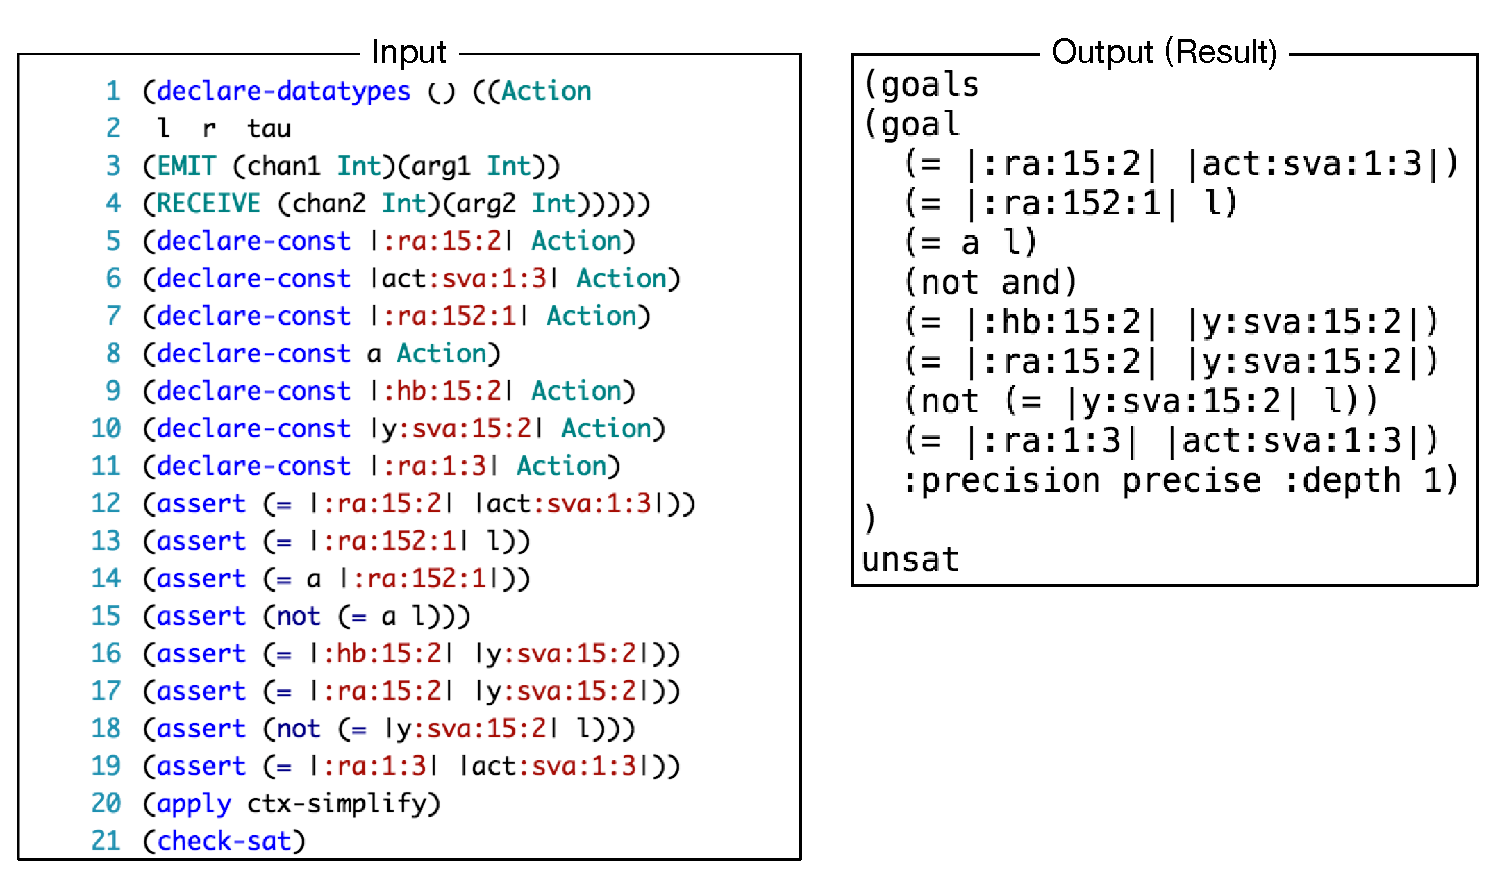
\includegraphics[width=10cm]{XFIG/SMTLIB1}}
  \caption{The input of the Z3 solver in SMT-LIB language and the output result}  \label{schema:smt-lib}
\end{figure}

\begin{figure}[t]
  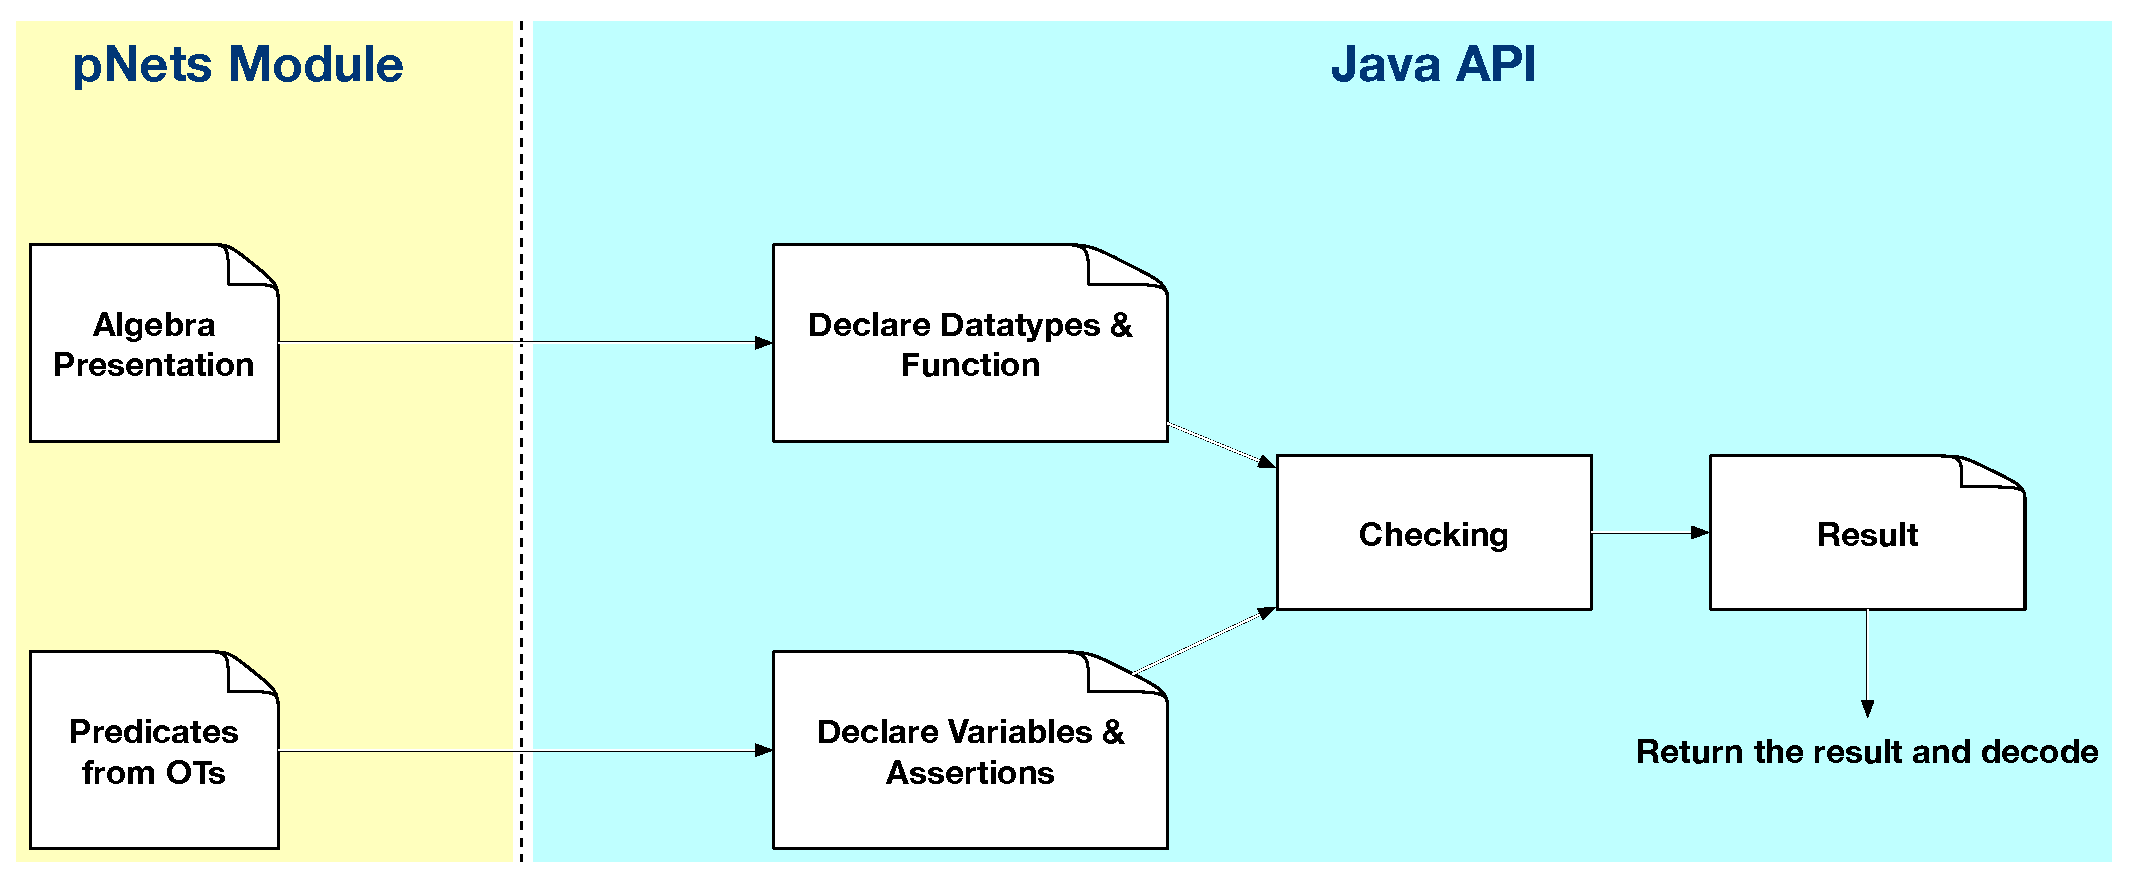
\includegraphics[width=\linewidth]{XFIG/Interaction}
  \caption{The architecture of the interaction between pNet API and Z3}  \label{schema:interaction}
\end{figure}

\paragraph{Interaction with Z3}
%\TODO{1. example input of Z3 in SMT-LIB.[DONE] 2. software architecture.[DONE]}
There are several ways to interact with the Z3 solver. 
It is possible to use Z3 interactively using the SMT-LIB
(Python-based) language. From inside our algorithm code, 
we implement the dynamic interaction between the pNet API and Z3
solver through its JAVA API. But here we present the code in Z3 by
SMT-LIB language instead of JAVA codes to make it easier to read. In
Fig~\ref{schema:smt-lib}, we show the  input of the unsatisfiable
result before.
The input starts with the declaration of the CCS action algebra types
and constructors.
Some $datatypes$ are declared to input the sorts of the CCS example, here we only declare one $datatypes$ named $Action$ to involve all the constant actions. The $Int$ and $Bool$ are already existed in Z3. Then we input the predicate of that open transition in two parts. The variables contained in the predicate are declared first, then the terms of predicate are inputed as $assertions$ one by one. In the output, "(not and)" shows Z3 have found out the contradiction in the predicate and the result "unsat" is just what we expected.  



We present the architecture of the interaction with Z3 in
Fig~\ref{schema:interaction}.
For each OT generated at the toplevel of a pNet, the predicate must be
submitted for satisfiability check to Z3. For that we need to
translate into Z3 (Java-API) syntax, both the elements of the action
algebra, and the predicates itself, including the encoding of the
variable assignments (the Post part).

The $presentation$ of the action algebra
is declared at the beginning of the algorithm as the $sorts$ and the
$operators$ will be used throughout the whole algorithm. It is
translated into $datatypes$ and $functions$ then submitted to the Z3
at the same time. Each candidate predicate will then be translated into $assertions$ before submitted to Z3 after the algorithm computing out all the possible open transitions, they act as intermediate results there. Together with the $datatypes$ and $functions$, the $assertions$ are used to check the satisfiability of the predicate in Z3.


\paragraph{Translation of Action algebra presentation}

The $datatypes$ are declared according to the $sorts$ the users declared in the $presentation$. If the return type of the $functions$ is one of the $datatypes$, we add this $function$ when declare the $datatypes$, it present the reality that every action expression also belongs to a sort of pNet. 

\QIN{
So when we declare the operator EMIT we illustrated in section 4.1, it will be just declared together with the constants.
}

 Although in Fig~\ref{schema:smt-lib} we have not declared $functions$, they should be exactly declared if there are new $operators$ declared in the $presentation$. The input type of the $function$ can be $Int$, $Bool$ or the $datatypes$ declared all determined by the construct of the  $operators$ in the presentation. For example, we define a new operator to present the equation between two actions in CCS example $\text{EQUAL}$ in the format likes:

\[< Action , Action > \rightarrow Bool .\]

It will be translated into the Z3 statement: 

\[\text{(declare-fun\ EQUAL\ (Action\ Action)\ Bool) .}\]

\paragraph{Translating assignments into predicate terms}

The assignments are also taken into account when checking the
satisfiability of the open transitions as they represent the value of
the variables involved in an OT. In order to do that, we employs a
translation from assignments into term of predicates. The assignments
required to be translated are only those belong to the variables
contain in the start states of the open transitions. The assignments
are represented as equations between the variables and the expressions
on the right side of assignment. For the assignments of the same
variable, we do not figure out which state is the precursor of current
state, we keep all these possible equations instead, and generate the
disjunction of these equations. The state could always move to the
target state if there exists one of the values of its variable
satisfies the guard.
%\TODO{It won't matter the variable of the next state
%except that the right hand side expression contain its variables. This
%is a problem left to be solved in our future work. WHICH PROBLEM ?}
After that, for the assignments of the different variables, we generate a conjunction of them. This way we obtain a new term of the predicate involving assignments of the variables.


\paragraph{checking satisfiability}

% We check the satisfiability of open transitions on the top level of
% the pNet, treating these open transitions as the intermediate result
% of the algorithm. After we get the intermediate results of open
% transitions, we check them one by one.
Here we declare the variables in the predicate first to make Z3 know all the parameters used for checking this time. The variable including the argument in the operators must has its sort as every pNet defines two default sorts $Int$, $Bool$ default and at least one sort for the actions. The variables can declared using the $datatypes$ declared in the format as:

\[\text{(declare-const\ a\ Action) .}\]

The predicate submitted to the Z3 contain the assignments as them
become a part of predicate after our translation. Each term of the
predicate is an assertion in Z3, as an example, in the former
unsatisfiable result in Fig~\ref{schema:unsat-ot}, the contradiction is occured in terms: 

\[(:ra:152:1 = l) \land (a = :ra:152:1) \land (l \neq a) .\]

from which we generate the following three assertions:

\[\text{(assert\ (=\ |:ra:152:1|\ l))}\ \ \ \text{(assert\ (=\ a\ |:ra:152:1|))}\ \ \ \text{(assert\ (not\ (=\ a\ l)))}\]

\subsection{Result of the running example}
\label{section:full-result}
% \TODO{
% Xudong: full result of the tool execution on the running example\\\\
% Open Automata of the CCS example.

We get the final result after pruning all the unsatisfiable open
transitions, that is 2/3 of the intermediate results; the resulting open
automaton is shown in Fig.~\ref{schema:ccs-result}, we have drawn
manually the open automaton obtained as the final result generated by
algorithm.
The $ot_1$ represents the
value-passing between $a.P$ and $b.Q$ and they are synchronized then
give out an silent action $\tau$, process $P$ and $Q$ should not work
in this case. The $ot_3$ and $ot_5$ represent another possible path to
execute $a.P||b.Q$, action $a$ and $b$ are finished in sequence
instead of synchronizing, they are just transmitted out as the
external action. The behavior of the processes, presented as holes $P$
and $Q$ in this pNet, is uncertain, we only know the sort $Action$ for
them. So the action from $P$ might be synchronized with the action $b$
that is what $ot_9$ presents or be directly transmitted to the
external as the $ot_7$ shows. And we can see more cases of the
interaction between these two processes in the open transitions starting at
the state $11$, synchronizing two actions like $ot_{13}$ or directly
transmitting like $ot_{15}$. 

To sum up, from the pNet encoding CCS formula inputed by the user we
generate the open transitions and prune the unsatisfiability
automatically. The final result open transitions represent all the
possible movements of the CCS example. They can exactly construct the
open automaton for the given example.


\begin{figure}[h]
  \centerline{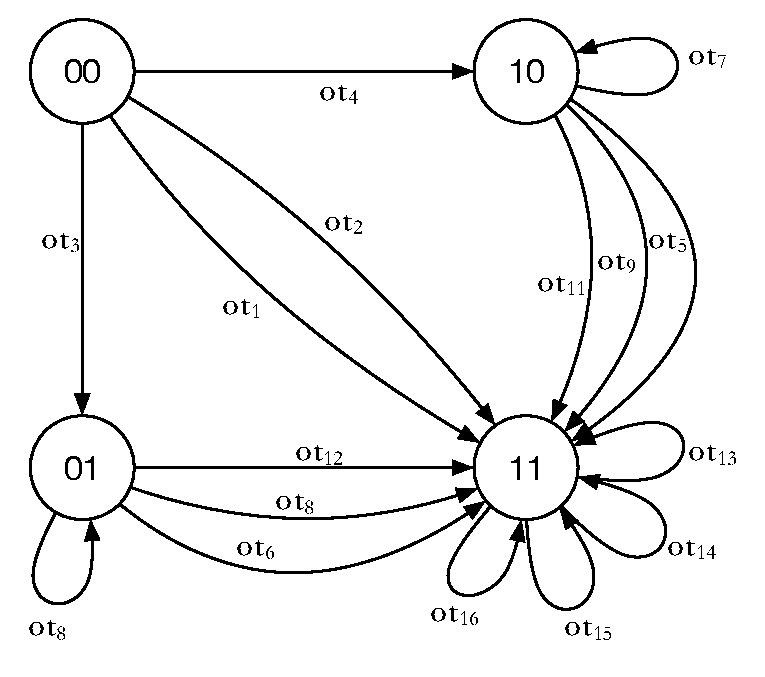
\includegraphics[width=7cm]{XFIG/CCSresult}}
  
$\begin{array}{@{}r@{}l@{}}
    ot_1  = &\openrule{\{0 \xrightarrow{a}_{C_1} 1, 0 \xrightarrow{b}_{C_2} 1\}, ~~a=!ch_{11}(v_{11}) \!\land\! b=?ch_{11}(v_{11}) \!\land\! a\neq l \!\land\! b\neq r\!\land\! v_1=\tau}
    {\ostate{00} \xrightarrow{v_1} \ostate{11}}\\
  \end{array}$
  
  \begin{minipage}{6cm}
$\begin{array}{@{}r@{}l@{}}
    ot_3  = &\openrule{\{0 \xrightarrow{a}_{C_1} 1\}, ~~a\neq l \!\land\! v_3=a}
    {\ostate{00} \xrightarrow{v_3} \ostate{10}}\\
    ot_5  = &\openrule{\{0 \xrightarrow{b}_{C_2} 1\}, ~~b\neq r \!\land\! v_5=b}
    {\ostate{10} \xrightarrow{v_5} \ostate{11}}\\
  \end{array}$
  \end{minipage}
   \hspace{2mm}
  \begin{minipage}{6cm}
$\begin{array}{@{}r@{}l@{}}
    ot_7  = &\openrule{\{1 \xrightarrow{l}_{C_1} 1\}, ~~\{\xrightarrow{hb_{17}}\}, ~~v_7=hb_{17}}
    {\ostate{10} \xrightarrow{v_7} \ostate{10}}\\
  \end{array}$
  \end{minipage}
    
$\begin{array}{@{}r@{}l@{}}
    ot_9  = &\openrule{\{0 \xrightarrow{b}_{C_2} 1\}, ~~\{\xrightarrow{hb_{19}}\}, ~~b=!ch_{19}(v_{19}) \!\land\! b\neq r \!\land\! hb_{19}=?ch_{19}(v_{19})\!\land\! v_9=\tau}
    {\ostate{10} \xrightarrow{v_9} \ostate{11}}\\
  \end{array}$

$\begin{array}{@{}r@{}l@{}}
    ot_{13}  = &\openrule{\{1 \xrightarrow{l}_{C_1} 1, 1 \xrightarrow{r}_{C_2} 1\}, ~~\{\xrightarrow{hb_{113}}, \xrightarrow{hb_{213}}\}, ~~hb_{113}= !ch_{113}(v_{113}) \!\land\! hb_{213}=?ch_{113}(v_{113}) \!\land\! v_{13}=\tau}
    {\ostate{11} \xrightarrow{v_{13}} \ostate{11}}\\
  \end{array}$

$\begin{array}{@{}r@{}l@{}}
    ot_{15}  = &\openrule{\{1 \xrightarrow{l}_{C_1} 1\}, ~~\{\xrightarrow{hb_{115}}\}, ~~v_{15}=hb_{115}}
    {\ostate{11} \xrightarrow{v_{15}} \ostate{11}}\\
  \end{array}$

\caption{The open automaton of the CCS formula a.P||b.Q (a part of open transitions is shown)}  \label{schema:ccs-result}
\end{figure}



\section{Conclusion and Discussion}
\label{section:conclusion}

In this paper we presented the algorithm for generating an open
automaton representing the semantics of an open pNet, and we described
the implementation of the
algorithm. Our implementation includes two main parts. First, we
compute all the possible open transitions. The actions in pLTS and
hole behaviors are composed in the algorithm while the generation of
predicate need to match the combinations of the subnets with the
synchronization vectors. Some of the open transitions obtained at this
intermediate step, constructed in a structural manner from all
possible combinations of possible logical predicates, may
contain predicates which do not represent any possible concrete
instanciations. 
To get rid of these useless transtions, we use a SMT solver Z3 for checking the
satisfiability of the predicate in each open transition. In
order to do that, we have done some translation on the presentation,
the predicate and the assignments of the variables which are also
considered as a part of predicates before submitting them to the
Z3 solver. We implemented our algorithm in the VerCors platform and use some
running examples, the formula from other process algebras, to test the
algorithm. The result of the running examples are shown as the open
automaton with all the parameters generated by the algorithm
automatically. The open automaton successfully presents all the
possible movements of the CCS expression.   

Among the questions arising during this work, an important one is the
efficiency of Z3 for our needs. Z3 is famous for being very fast for
solving very large sets of assertions, and this could be important for
us. But we encountered  some problems during the implementation the
checking method using Z3. For example, if the $functions$ and the
$datatypes$ part of the algebra presentation we submit to the solver
are independent with each other, then checking the $assertions$ is a
simple work. However, $functions$ on recursive $datatypes$ make it
more complex, some special rules might be defined by user for the
induction. Also, we need more evidence that dealing with more complex
action algebras, that would involve axiomatizing their dat structures
into Z3 theories, will indeed allow us to decide validity of
predicates.
We may also try other automatic theorem provers, depending on th
estructure of the proofs we need.

Naturally, the next work after the generation of the open automata
will be to check the bisimulation of the pNets. In previous paper, we
have already found the FH-bisimulation, inspired by~\cite{deSimone85} as a
suitable definition. Usual approaches of bisimulation by partition
refinement does not work easily with symbolic transitions. In a first
step we may want instead to define and implement an algorithm fo
rchecking that a given equivalence relation between open automata
states is indeed a FH-Bisimulation. Finding automaticaly a
bisimulation relation or the most general bisimulation will be more
challenging. It appears also that when comparing different pNets with
different structure, strong bisimulation will be too strong a notion,
and that we will have to define proper notinos of weak equivalence or
refinements. 

Before that work, we need to reconsider the result open transitions
from our algorithm. The ideal
result that we showed in the bottom part of
Fig.~\ref{schema:ccs-result} is not the one generated by the algorithm,
because it contains many intermediate
variables, such as fresh local variables of synchronization
vectors, and fresh result variables of intermediate open transitions.
Such intermediate variables come from the way predicates are
generated, and depends on the particular structure of the pNet. But
they are not significant in the resulting behavior, and should be
eliminated before comparing such behavior with another pNet.
To eliminate the intermediate variables in the predicate, we want to define
the set of the significant variables that we won't eliminate: the
local variables of pLTS transitions, the hole behaviors and the result
action at the top level.
The result of the elimination will be simpler predicates, that can be
successfuly compared (e.g. by Z3) within the bisimulation checking
algorithm.



\bibliographystyle{lncs/splncs}

% \bibliography{oasis,biblio}
\bibliography{biblio}

% \newpage
% \appendix

\end{document}
